\documentclass[12pt,a4paper]{article}
\usepackage[polish]{babel}
\usepackage[T1]{fontenc}
\usepackage[utf8x]{inputenc}
\usepackage{hyperref}
\usepackage{url}
\usepackage{graphicx}
\usepackage{listings}
\usepackage{amsmath}
\usepackage{indentfirst}
\usepackage[]{algorithm2e}
\addtolength{\hoffset}{-1.5cm}
\addtolength{\marginparwidth}{-1.5cm}
\addtolength{\textwidth}{3cm}
\addtolength{\voffset}{-1cm}
\addtolength{\textheight}{2.5cm}
\setlength{\topmargin}{0cm}
\setlength{\headheight}{0cm}

\begin{document}
	
	\title{Dokumentacja projektu\\ Języki Skryptowe}
	\author{Konrad Lubera, gr 1A}
	\date{\today}
	
	\maketitle
	\newpage
	\section*{Część I}
	\subsection*{Opis programu}
	 Projekt spełnia warunki zadania Szyfrowanie Wiadomości z konkursu Algorytmion2015, dodatkowo obsługiwany jest z poziomu powłoki systemu Windows(skrypt batchowski) oraz wyświetla wyniki wykonanych operacji na stronie internetowej. 
	 \\
	\\ Poniżej polecenie z konkursu Algorytmion:
	
	Adam i Janek ustalili między sobą, że każdą wiadomość tekstową, będą szyfrować przy pomocy następującego sposobu:
	\begin{itemize}
	\item   Każdą literę i znak interpunkcyjny należy zamienić na odpowiadającą liczbę kodu ASCII (liczba naturalna od 0 do 127).
	\item Pierwsza, tak powstała liczba, jest zamieniana na system dwójkowy.
	\item Kolejne liczby, wynikające z kodu ASCII, są zamieniane na system liczbowy, który jest równy powiększonej o dwa reszcie z dzielenia przez osiem poprzedniej liczby.
	\item  Ilość cyfr zamienionej liczby, dla każdego systemu liczbowego, wynika z ilości cyfr zamiany liczby maksymalnej, czyli liczby 127 (dla systemu binarnego jest to siedem cyfr). 
	\end{itemize}
	Twoim zadaniem jest napisanie programu, który szyfruje i deszyfruje wiadomości. \\
Szyfrowanie tekstu z pliku tekst.txt do pliku szyfr.txt \\ Deszyfrowanie tekstu z pliku szyfr.txt do pliku odszyfrowane.txt 

	\subsection*{Instrukcja obsługi}
	Aby uruchomić program należy otworzyć plik server.bat znajdujący się w głównym folderze projektu, następnie wybrać opcje Uruchom wpisując 1 na klawiaturze oraz wcisnąć klawisz enter.
		
			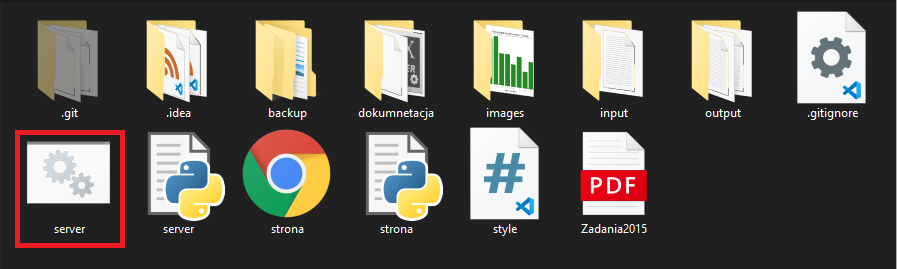
\includegraphics[scale=0.7]{instrukcja}

			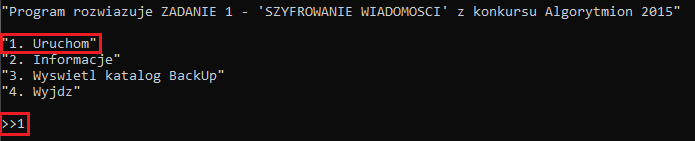
\includegraphics[scale=0.8]{instrukcja2}
	
	
\newpage
	\section*{Część II}
	\subsection*{Część techniczna}
	Schemat działania i szczegółowy opis komponentów, mechanizmów (bez kodu).
	\subsection*{Opis działania} 
Główny algorytm programy szyfruje podane słowa za pomocą zamiany kodu ASCII liter danego słowa z systemu dziesiętnego na odpowiednio wyliczony system liczbowy. Kod pierwszej litery jest zamieniany zawsze na system dwójkowy, system na który zamieniana jest kolejna litera obliczany jest według wzoru: $$sys=(l-1\mod{8})+2$$ 


sys - system liczbowy


l-1 - kod ASCII poprzedniej litery \\

Działanie to jest wykonywane w pętli do końca słowa. Sam algorytm zamiany systemów liczbowych opiszę w następnym rozdziale. Odszyfrowanie słów jest wykonywane przy użyciu tego samego działania, różnica jest taka że najpierw musimy musimy dokonać konwersji a później obliczyć system w szyfrowaniu natomiast najpierw obliczamy system a później dokonujemy konwersji. 
	\subsection*{Implementacja}
	Tutaj opisujemy wybrane działanie KODU programu -- z uwzględnieniem PSEUDOKODU (utworzonego przy użyciu \LaTeX, a nie obrazka).
	\begin{verbatim}
	proszę zwrócić uwagę na wychodzenie poza obszar kartki.
	\end{verbatim}
	\newpage
	\section*{Pełen kod programu}

	\begin{itemize}
	\item SERVER.PY
	\begin{lstlisting}[language=Python]


	\end{lstlisting}

	\item STRONA.PY
	\begin{lstlisting}[language=Python]

	\end{lstlisting}
	
	\item STRONA.HTML
	\begin{lstlisting}[language=Html]

	\end{lstlisting}
	
	\item STYLE.CSS
	\begin{lstlisting}

	\end{lstlisting}
	\end{itemize}

\end{document}
